\documentclass[tikz,convert={outfile=\jobname.svg}]{standalone}
%\usetikzlibrary{...}% tikz package already loaded by 'tikz' option
\begin{document}

%\newcommand*{\xMin}{0}%
%\newcommand*{\xMax}{12}%
%\newcommand*{\yMin}{0}%
%\newcommand*{\yMax}{8}%
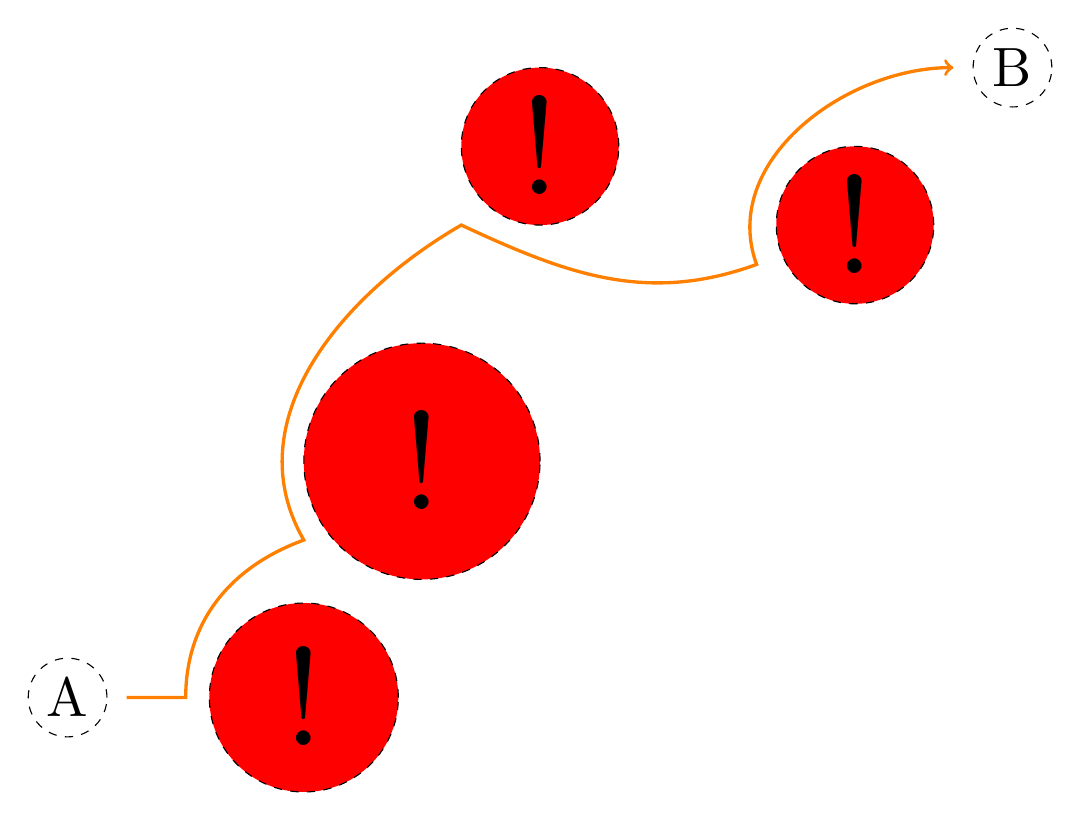
\begin{tikzpicture}

%	\foreach \i in {\xMin,...,\xMax} {
%        \draw [very thin,gray] (\i,\yMin) -- (\i,\yMax)  node [below] at (\i,\yMin) {$\i$};
%    }
%    \foreach \i in {\yMin,...,\yMax} {
%        \draw [very thin,gray] (\xMin,\i) -- (\xMax,\i) node [left] at (\xMin,\i) {$\i$};
%    }
	
	\draw [dashed] (0,0) circle [radius=0.5];
	\draw (0,0) node[scale=2]{A};
	
	\draw [dashed] (12,8) circle [radius=0.5];
	\draw (12,8) node[scale=2]{B};
	
	\draw [dashed, fill=red] (3,0) circle [radius=1.2];
	\draw (3,0) node[scale=5]{!};
	
	\draw [dashed, fill=red] (4.5,3) circle [radius=1.5];
	\draw (4.5,3) node[scale=5]{!};
	
	\draw [dashed, fill=red] (6,7) circle [radius=1];
	\draw (6,7) node[scale=5]{!};
	
	\draw [dashed, fill=red] (10,6) circle [radius=1];
	\draw (10,6) node[scale=5]{!};
	
	\draw [->,very thick, orange] (0.75,0) to [out=0,in=180] (1.5,0) to [out=90,in=200] (3,2) to [out=120,in=-150] (5,6) to [out=-25, in=-160] (8.75,5.5) to [out=110, in=180] (11.25,8);
\end{tikzpicture}
\end{document}